\documentclass[11pt]{article}

\usepackage[margin=1in]{geometry}
\usepackage{fancyhdr}
\pagestyle{fancy}
\usepackage{graphicx}
\usepackage{adjustbox}
\usepackage{listings,lstautogobble}
\usepackage{courier}

\lstset{basicstyle=\footnotesize\ttfamily,
	breaklines=true,
	autogobble=true,
	language=SQL}


\lhead{CS 351 Assignment \#3 }
\chead{John Karasev}
\rhead{March 2, 2018}


\begin{document}

\section{Data}

        \adjustbox{valign=t}{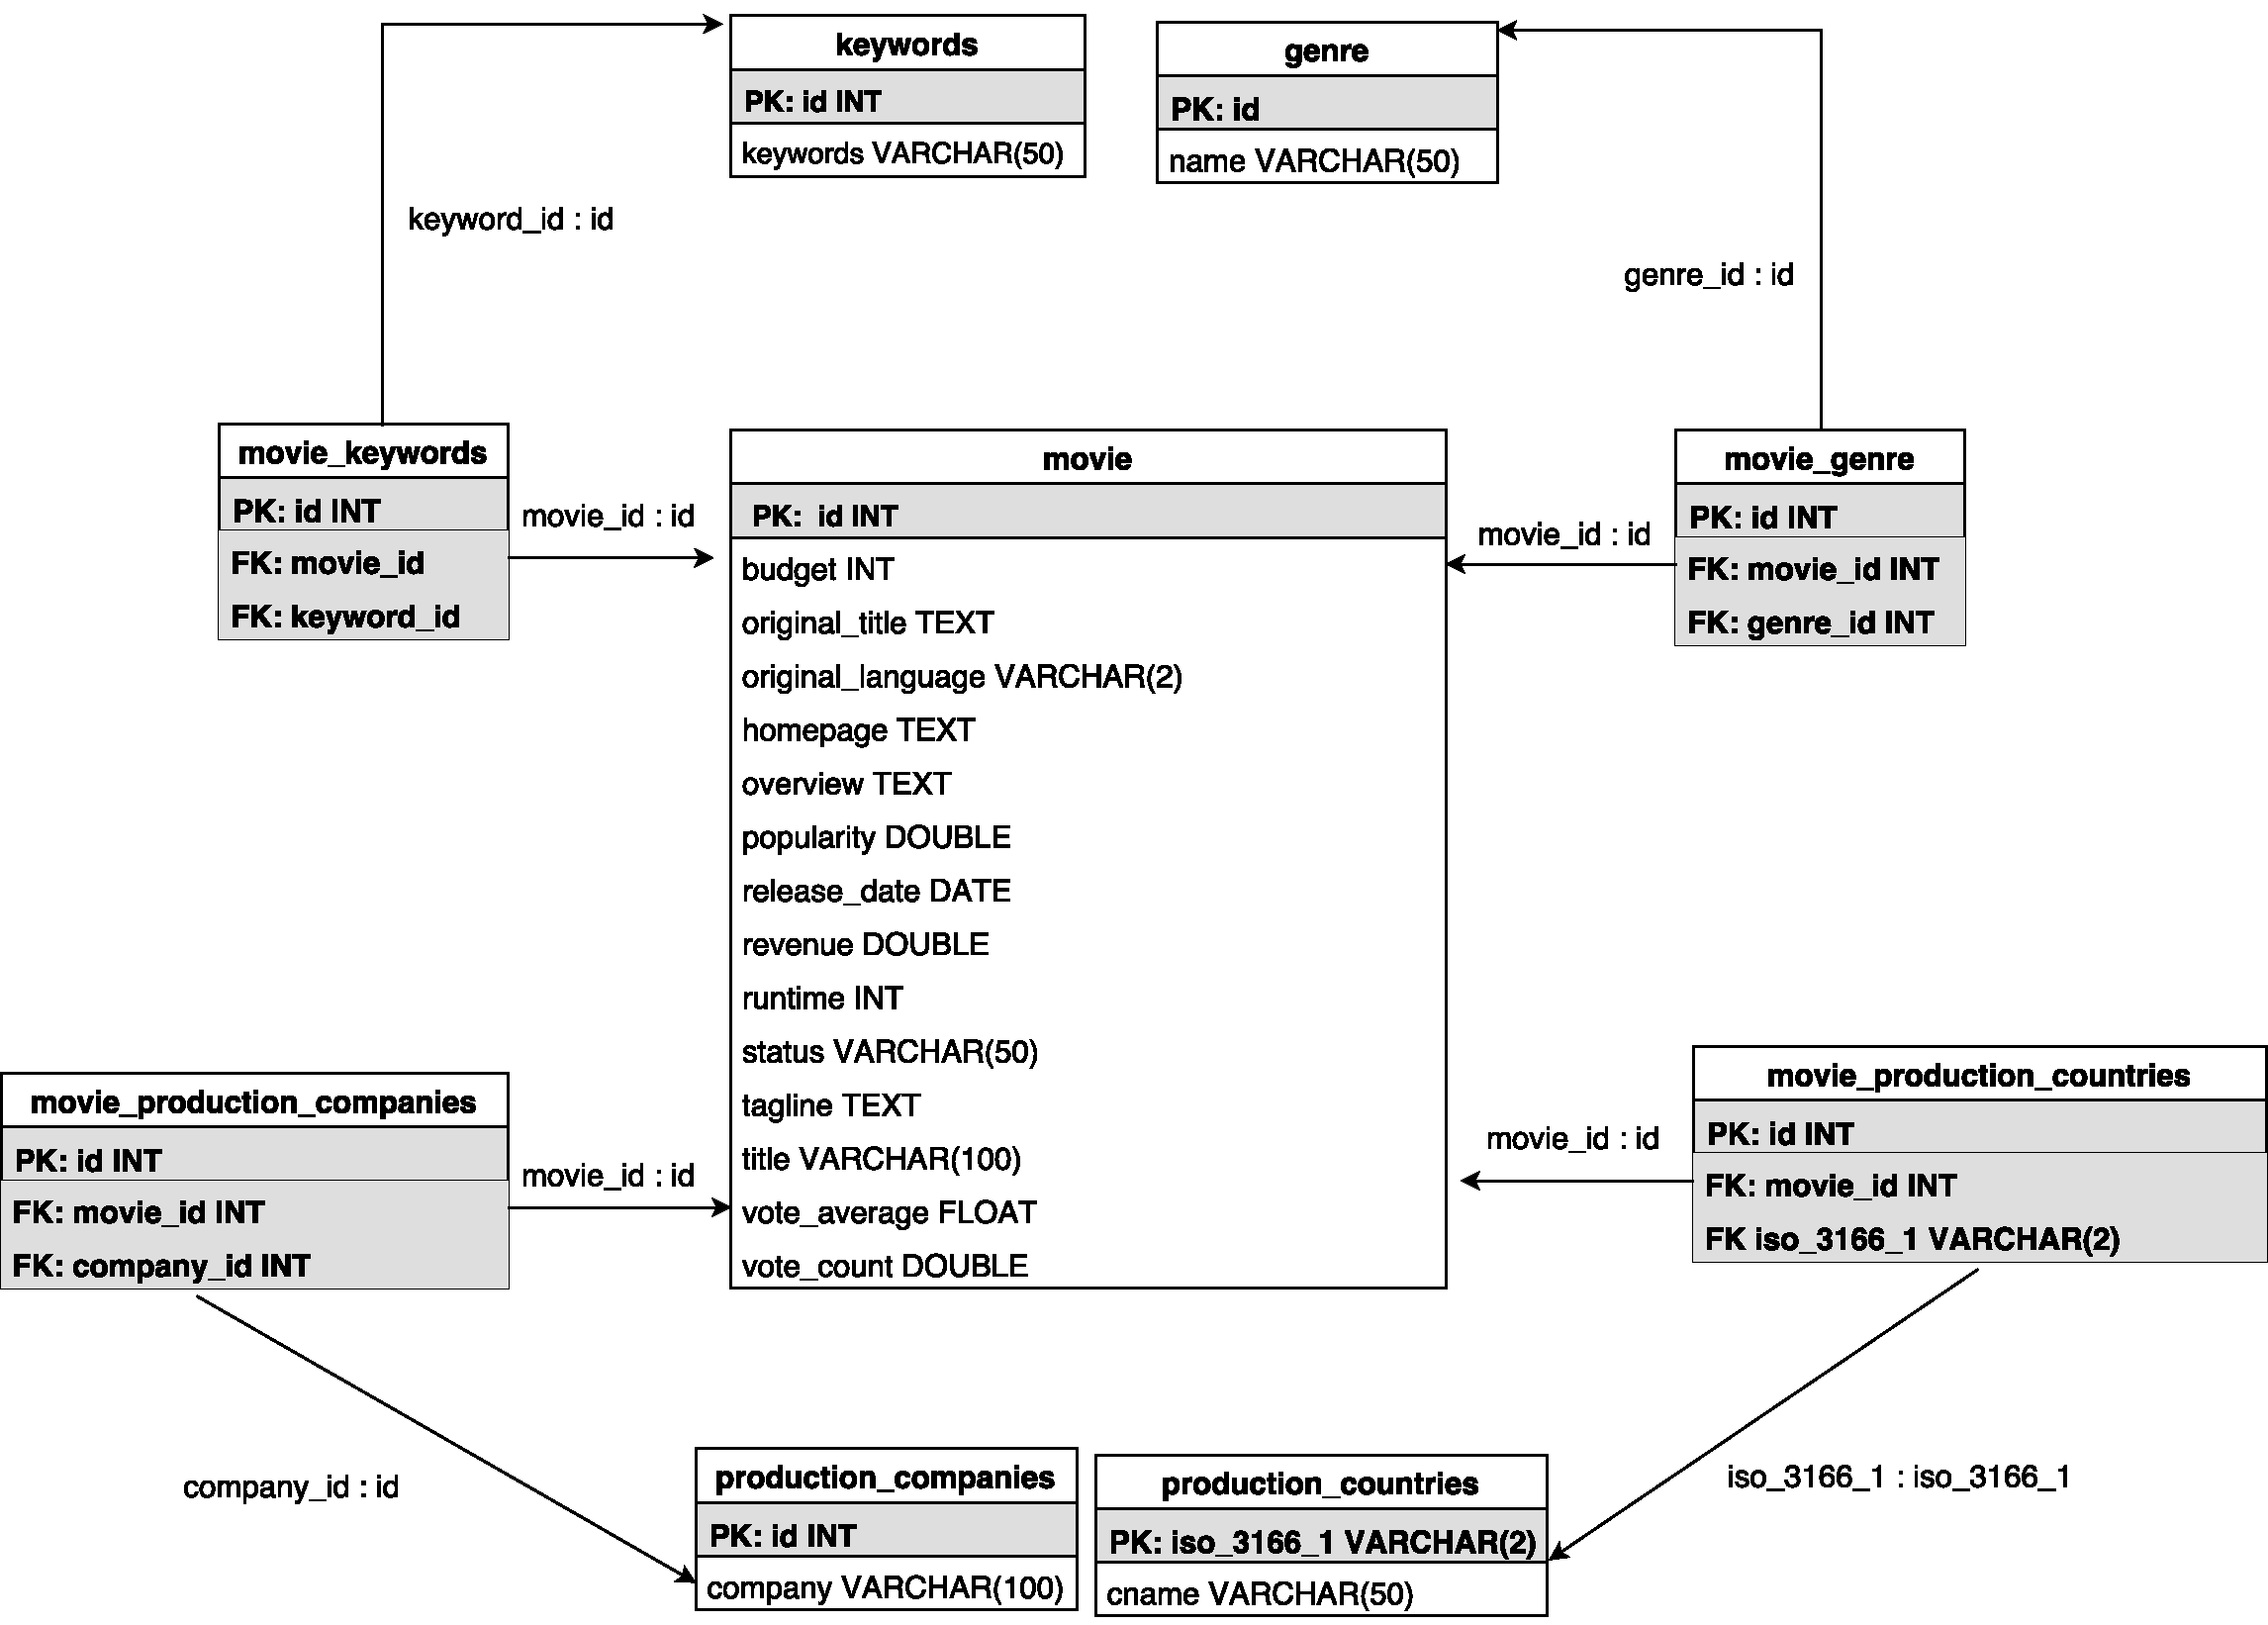
\includegraphics[width=15cm]{./figures/uml.pdf}}
	\vspace{2cm}\\
	Above are all the schemas and their relationships with other schemas.
	PK stands for primary key and FK stands for foriegn key. All the entries
	in the movies csv that where not atomic, I broke them down into two seperate tables.
	One those two tables I used to show the relationship to the \textbf{movie} table and the other
	one just kept specific information such as \textbf{keywords}, \textbf{genre}, and \textbf{production\_companies}.
	All tables are in BCNF because (1) all atributes are atomic, (2) all non-key attributes
	depend only on the candidate key, (3) and in all $X \rightarrow Y$ FD's, $X$ is a candidate
	key. For example, all atributes in the \textbf{movie} table only depend on the candidate key \textbf{id}.
\pagebreak
\section{Queries}
\begin{enumerate}
	\item
		\begin{lstlisting}
		SELECT avg(budget) FROM movie;
		\end{lstlisting}
  		\begin{tabular}{| c | }
    			\hline
    				29045039.8753 \\
    			\hline
  		\end{tabular}

	\item
		\begin{lstlisting}
		SELECT title, company
		FROM
	  	  (
	    	    SELECT title, company, iso_3166_1
	    	    FROM movie
	    	    INNER JOIN movie_production_countries
	    	    ON movie.id=movie_production_countries.movie_id
	    	    INNER JOIN movie_production_companies
	    	    ON movie_production_companies.movie_id=movie_production_countries.movie_id
	    	    INNER JOIN production_companies company
	    	    ON movie_production_companies.company_id = company.id
	  	  ) AS full
		WHERE full.iso_3166_1='US';
		\end{lstlisting}
		\begin{tabular}[t]{| l | r | }
			\hline
			Four Rooms & Miramax Films \\ \hline
			Four Rooms & A Band Apart \\ \hline
			Star Wars & Lucasfilm \\ \hline
			Star Wars & Twentieth Century Fox Film Corporation \\ \hline
			Finding Nemo & Pixar Animation Studios \\
			\hline
		\end{tabular}
	\item
		\begin{lstlisting}
		SELECT title, revenue
		FROM movie
		ORDER BY revenue DESC LIMIT 5;
		\end{lstlisting}
		\begin{tabular}[t]{| l | r | }
			\hline
			Avatar & 2787965087 \\ \hline
			Titanic & 1845034188 \\ \hline
			The Avengers & 1519557910 \\ \hline
			Jurassic World & 1513528810 \\ \hline
			Furious 7 & 1506249360 \\
			\hline
		\end{tabular}
	\pagebreak
	\item
		\begin{lstlisting}
                SELECT mys.title, genre.name
                FROM
                  (
                      SELECT title, g2.name, g.movie_id
                      FROM movie
                        INNER JOIN movie_genre g ON movie.id = g.movie_id
                        INNER JOIN genre g2 ON g.genre_id = g2.id
                      WHERE g2.name="Science Fiction"
                  ) AS sci
                  INNER JOIN
                    (
                      SELECT title, g2.name, g.movie_id
                      FROM movie
                        INNER JOIN movie_genre g ON movie.id = g.movie_id
                        INNER JOIN genre g2 ON g.genre_id = g2.id
                      WHERE g2.name = "Mystery"
                    ) AS mys
                  ON sci.movie_id=mys.movie_id
                  INNER JOIN movie_genre ON movie_genre.movie_id=mys.movie_id
                  INNER JOIN genre ON genre.id=movie_genre.genre_id;
		\end{lstlisting}
		\begin{tabular}[t]{| l | r | }
			\hline
			Tomorrowland & Adventure \\ \hline
			Tomorrowland & Family \\ \hline
			Tomorrowland & Mystery \\ \hline
			Tomorrowland & Science Fiction \\ \hline
			Inception & Action \\
			\hline
		\end{tabular}
	\item
		\begin{lstlisting}
		SELECT title, popularity
		FROM movie
		WHERE popularity > (SELECT avg(popularity) FROM movie);
		\end{lstlisting}
		\begin{tabular}[t]{| l | r | }
			\hline
			Four Rooms & 22.87623 \\ \hline
			Star Wars & 126.393695 \\ \hline
			Finding Nemo & 85.688789 \\ \hline
			Forrest Gump & 138.133331 \\ \hline
			American Beauty & 80.878605 \\
			\hline
		\end{tabular}



\end{enumerate}



\end{document}
